\chapter{Technology Stack}

La scelta della tecnologia da impiegare è un aspetto fondamentale di ogni progetto, e questo chiaramente non fa eccezione. \\

Molti testi --- fra cui uno dei preferiti dall'autore\footnote{Si tratta di \cite{pragmatic}, un libro estremamente interessante, oltre che essenziale come spunto di riflessione per lo sviluppo personale e professionale di ogni informatico che osi definirsi programmatore.} --- hanno proposto analogie fra gli utensili di un artigiano e gli strumenti software di un qualaunque utlizzatore informatico. Sull'onda di questa metafora, una lima non adatta al tipo di materiale che si intende lavorare non potrà mai garantire risultati eccellenti, indipendentemente dalla bravuta dell'artigiano stesso. \\

Appare chiaro che una scelta sbagliata di tecnologie da utilizzare può condizionare negativamente l'esito di un qualaunque lavoro, pertanto occorre prestare particolare attenzione nel decidere quale tecnologia impiegare per raggiungere lo scopo.

\section{Strumenti Necessari}

    Messi da parte i vaneggiamenti poetici, all'atto pratico è evidente che gli strumenti di cui l'analisi ha bisogno sono in realtà pochi e piuttosto comuni:

    \begin{itemize}
        \item abbiamo a che fare con una certa quantità di dati $\rightarrow$ servirà un \textit{Data Base Management System}.
        \item occorre avere una comprensione generale dei dati $\rightarrow$ occorrerà un software che permetta di usare \textit{tecniche di visualizzazione}.
        \item dobbiamo lanciare degli algoritmi di \textit{data mining} $\rightarrow$ abbiamo bisogno di un software che li implementi.
    \end{itemize}

    Tutto questo è facilmente ottenibile impiegando gli strumenti che saranno descritti nelle prossime sezioni.

\section{Data Base Management System: MongoDB}

    \begin{figure}
        \centering
        \caption{logo del DBMS MongoDB}
        \label{mongodb_logo}
    	
\includegraphics[scale=0.70]{img/mongodb.png}
    \end{figure}

    La scelta del Data Base Management System è stata quella che ha impattato più di tutte il tipo di lavoro che è stato necessario fare.

    \subsection{La scelta di MongoDB}
    
        Sono state valutati principalmente due \textit{DBMS} candidati, entrambi \textit{open source}:

        \begin{itemize}
            \item \textbf{MySQL}, un \textit{DBMS} relazionale, rodato e ormai \textit{staple} nella manipolazione dati
            \item \textbf{MongoDB}, un \textit{DBMS} di nuova generazione che adotta invece il paradigma \textit{NoSQL} 
        \end{itemize}

        I dati che si hanno a disposizione sono in forma ovviamente relazionale --- cioè, sono tabelle. Utilizzare \textit{MySQL} potrebbe sembrare quindi una scelta tanto solida quanto ovvia, ma sul piano prestazionale il \textit{modello a documenti} di \textit{MongoDB} risulta sensibilmente più efficiente nel manipolare grandi quantità di dati molto diversi fra loro. \\

        La decisione che è stata infine presa --- \textit{utilizzare MongoDB} --- ha tenuto conto anche del valore didattico che ha l'imparare un nuovo paradigma di memorizzazione dati che trascende il classico modello relazionale.

    \subsection{Caratteristiche di MongoDB}

        Come si può banalmente leggere in \cite{mongowiki}: \\
        
        "\textbf{MongoDB} \textit{(da "humongous", enorme)} è un DBMS non relazionale, orientato ai documenti. Classificato come un database di tipo \textbf{NoSQL}, MongoDB si allontana dalla struttura tradizionale basata su tabelle dei database relazionali in favore di \textbf{documenti in stile JSON} con schema dinamico (MongoDB chiama il formato BSON), rendendo l'integrazione di dati di alcuni tipi di applicazioni più facile e veloce." \\

        La società MongoDB Inc mette a disposizione liberamente e gratuitamente una buona documentazione in \cite{mongodb}, la quale contiene tutte le informazioni necessarie per utilizzare almeglio il DBMS da loro sviluppato. 

        Oltre alla sua \textit{shell}, MongoDB espone delle \textit{API} per i principali linguaggi di programmazione. Questo aspetto è tornato molto utile per specificare le operazioni di \textit{preprocessing} in un linguaggio familiare e più facilmente gestibile del dialetto di Javascript nativo di MongoDB.

\section{Interazione col DBMS: Python}

    \begin{figure}
        \centering
        \caption{logo del linguaggio di programmazione Python}
        \label{python_logo}
    	
\includegraphics[scale=0.1]{img/python.png}
    \end{figure}

    A proposito di quando detto alla fine della sezione precedente, il linguaggio scelto è stato \textbf{Python}. Come si può leggere direttamente da \cite{pywiki}:\\

    "\textit{Python} è un linguaggio multi-paradigma, che ha tra i principali obiettivi \textit{dinamicità}, \textit{semplicità} e \textit{flessibilità}. Supporta il paradigma object oriented, la programmazione strutturata e molte caratteristiche di programmazione funzionale e riflessione." \\

    Il linguaggio Python ha una estesa e approfondita documentazione, messa a disposizione direttamente dalla Python Software Foundation in \cite{python}.

    \subsection{API per MongoDB: pymongo}

        \begin{figure}
            \centering
            \caption{schema riassuntivo del modello di lavoro con \textbf{pymongo}}
            \label{pymongo_logo}
    	    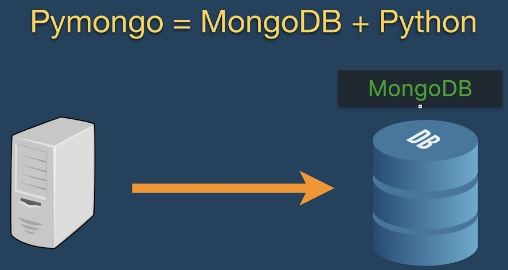
\includegraphics[scale=0.75]{img/pymongo.png}
        \end{figure}

        Una sintetica ma tremendamente efficace descrizione di che cosa è \textbf{pymongo} si può trovare direttamente nella sua documentazione, in \cite{pymongo}:\\

        "PyMongo is a Python distribution containing tools for working with MongoDB, and is the recommended way to work with MongoDB from Python." \\

        Che tradotto in italiano sgnifica: \\

        "PyMongo è una distribuzione di Python che contiene degli strumenti per lavorare con MongoDB, ed è la maniera raccomandata per avere a che fare con MongoDB da Python." \\

        In altre parole, \textbf{pymongo} è una libreria per python che fornisce oggetti e metodi per lanciare istruzioni di \textit{Data Definiion}\footnote{Data Definition Language: sottoinsieme di un linguaggio comprendente le istruzioni per definire e manipolare le strutture (in un DBMS relazionale, le \textit{tabelle}, in MongoDB le \textit{collezioni} di documenti). Ad esmepio, in \textbf{SQL} comprende le istruzioni \textbf{create table}, \textbf{alter table}, \ldots} e \textit{Data Manipulation}\footnote{Data Manipulation Language: sottoinsieme di un linguaggio comprendente le istruzioni per manipolare i dati. Ad esmepio, in \textbf{SQL} sono ad esempio \textbf{insert}, \textbf{update}, \ldots}.

\section{Algoritmi di Data Mining: Weka}

        \begin{figure}
            \centering
            \caption{logo di Weka}
            \label{weka}
    	    
\includegraphics[scale=0.75]{img/weka.png}
        \end{figure}

    Come si può leggere direttamente da \cite{wekawiki}, "\textbf{Weka}, acronimo di \textbf{W}aikato \textbf{E}nvironment for \textbf{K}nowledge \textbf{A}nalysis, è un software per l'apprendimento automatico sviluppato nell'università di Waikato in Nuova Zelanda. È open source e viene distribuito con licenza \textit{GNU General Public License}. Curiosamente la sigla corrisponde al nome di un simpatico animale simile al Kiwi, presente solo nelle isole della Nuova Zelanda." \\

    Sempre secondo \cite{wekawiki}, "Weka è un ambiente software interamente scritto in Java. Un semplice metodo per utilizzare questo software consiste nell'applicare dei metodi di apprendimento automatici (learning methods) ad un set di dati (dataset), e analizzarne il risultato". \\

    Nel merito del nostro lavoro, Weka è una \textit{suite} di sottoprogrammi molto potente, che permetterebbe di effetturare ogni aspetto del processo di \textit{data mining}, dal \textit{preprocessing} al \textit{postprocessing}. Ai fini de nostro scopo, questo software verrà utilizzato principalmente come ambiente per lanciare gli algoritmi implementati dalle sue librerie. Come si può vedere consultando la sua estesa documentazione in \cite{weka}, Weka può essere integrato in un gran numero di ambienti; tuttavia, per questa applicazione è stato scelto di utilizzarlo in forma \textit{stand alone}, preferendo concentrarsi sul merito delle analisi da fare e lasciando perdere il lavoro di programazione che sarebbe seguito da scelte diverse.\\

\section{Tecniche di Visualizzazione}

    \subsection{Linguaggio R}

        \begin{figure}
            \centering
            \caption{logo di R}
            \label{R}
    	    
\includegraphics[scale=0.75]{img/R.png}
        \end{figure}

        Direttamente dalla pagina Wikipedia relativa al sotware R (in \cite{Rwiki}), "R è un linguaggio di programmazione e un ambiente di sviluppo specifico per l'analisi statistica dei dati. [...] È un software libero in quanto viene distribuito con la licenza GNU GPL, ed è disponibile per diversi sistemi operativi (ad esempio Unix, GNU/Linux, macOS, Microsoft Windows). Il suo linguaggio orientato agli oggetti deriva direttamente dal pacchetto S [...]." \\

        Un'estesa ed approfondita documentazione può essere trovata in \cite{R}. Come si può notare consultandola, le potenzialità di questo software sono molto vaste; nel merito di questo studio è stato usato solamente una minuscola frazione delle funzioni offerte --- ovvero la realizzazione di grafici a partire da un set di dati --- perciò, analogamente a quanto osservato riguardo a Weka, è stato scelto di non spendere troppo tempo nell'integrazione di questo strumento in un flusso di automazione ma di usarlo soltanto in forma a sé stante.\\

    \subsection{Fogli di Calcolo}

    Per quanto banale possa sembrare, per alcuni dati molto semplici può essere utile non andare a scomodare strumenti troppo complessi, impiegando invece attrezzi dall'utilizzo estremamente semplice, come un foglio di calcolo. \\

    A questo proposito, è stato scelto di utilizzare Calc (\cite{calc}), facente parte della \textit{suite da ufficio} LibreOffice, un progetto open source che is pone come alternativa a Microsoft Office. \\

    Con esso è stato possibile realizzare semplici grafici di data set dalla mole ridotta, senza incorrere nell'\textit{overhead} --- inteso come carico di lavoro necessario a raggiungere un risultato simile --- che avrebbe comportato l'utilizzo di R.

\section{Redazione di questo documento}

    Per quanto scontato e irrilevante possa sembrare, una parte integrante del lavoro svolto è stato quello di redarre questo documento. Vista in quest'ottica, appare chiaro che la scelta di uno strumento adatto possa condizionare in positivo la chiarezza e l'efficacia di questa produzione scritta. \\

    Dato che lo standard accademico impone l'utilizzo del \LaTeX per questo genere di lavori, è stata scelta una distribuzione aggiornata e supportata di esso, \textbf{TeX Live}, ottenuta direttamente dalle repository di Arch Linux.

\section{Conclusioni}

    Volgendo uno sguardo generale a quanto scritto fino a ora, possiamo dire che la nostra technology stack si compone di un mix di strumenti vario e tutto sommato moderno. Alcuni di essi sono di stampo generalista, non specifici per il nostro campo di applicazione, ma comunque sufficientemente malleabili per poter essere impiegati adeguatamente. \\

    Riassumendo il tutto in pochi, semplici punti, la technology stack è la seguente:

    \begin{itemize}
        \item MongoDB come DBMS
        \item Python (pymongo) per manipolare i dati su MongoDB
        \item R e LibreOffice Calc per le tecniche di visualizzazione
        \item Weka per gli algoritmi di data mining
        \item TeX Live su Arch Linux come distribuzione \LaTeX
    \end{itemize}

    Ora che è ben chiaro cosa verrà utilizzato e a che scopo, si è in grado di cominciare finalmente il lavoro sui dati.
